\section{Phong Lichtmodell}
\begin{figure}[H]
	\centering
	\begin{tikzpicture}[scale=2]
	\draw (-1,0)--(1,0);
	\node[fill, circle, label={P}, scale=.25] (0,0) (P) {};
	\draw[dashed] (P) -- (2*-.951, 2*.309) node[rotate={-18}] {\varangle};
	\draw[dashed] (P) -- (2*.707, 2*.707) node {\textasteriskcentered};
	\draw[-latex] (P)--(0,1) node[label=n]{};
	\draw[-latex] (P) -- (.707,.707) node[label={$\ell$}] {};
	\draw[-latex] (P) -- (-.707,.707) node[label=r] (r) {};
	\draw[-latex] (P) -- (-.951, .309) node[label=v] (v) {};
	\draw pic["$\alpha$", draw, angle eccentricity=1.2, angle radius=1cm]
	{angle=r--P--v};
	\end{tikzpicture}
\end{figure}
\[ |n| = |\ell| = |r| = |v| = 1 \]
\[ r = 2n(n^T\ell) - \ell \]
S = Shininess
\[ I_S = I_L (\cos \alpha)^S = I_L\left( r^Tv \right)^S, ~~ I_D = I_L\left( n^T\ell \right) \]
\begin{figure}[H]
	\centering
	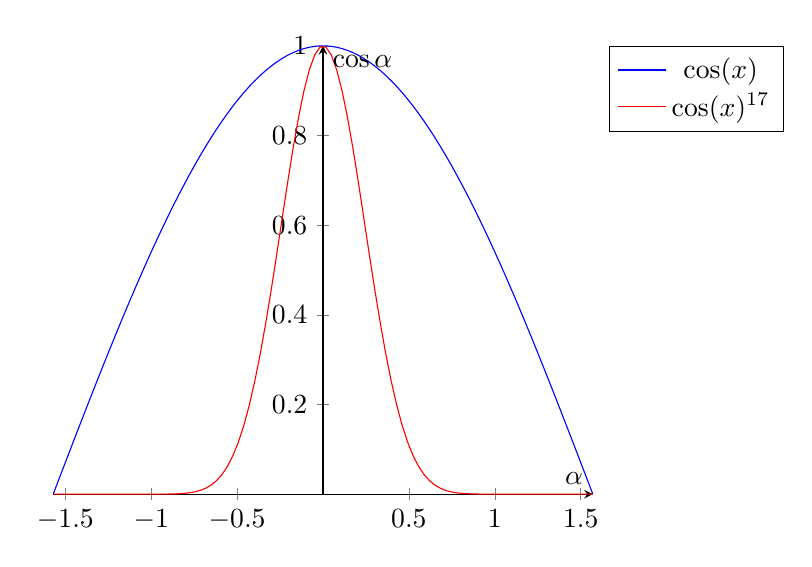
\begin{tikzpicture}
	\begin{axis}[xlabel={$\alpha$},ylabel={$\cos\alpha$}, domain=-pi/2:pi/2, samples=100, legend pos=outer north east, axis lines = center]
	\addplot[draw=blue] {cos(deg(x))};
	\addplot[draw=red] {(cos(deg(x)))^(17)};
	\legend{$\cos(x)$,$\cos(x)^{17}$,}
	\end{axis}
	\end{tikzpicture}
\end{figure}
\subsection{Phong}
\[ I_\text{Color} = I_\text{Ambient,Color} + I_\text{Diffuse,Color} + I_\text{Specular, Color} \]
\[ \text{Color} \in \left\{ \text{Red}, \text{Green}, \text{Blue}\right\} \]

\begin{lstlisting}[language=c++]
void main() {
	vec3 normal = normalize(vNormal);
	vec3 lightDir = normalize(lighPos - vPos);
	vec3 reflectDie = reflect(lightDir, normal);
	vec3 viewDir = normalize(-vPos);
	
	float lambertian = max(dot(loghtDir, normal), 0.0.);
	float specular = 0.0;
	
	if ( lambertian > 0.0) {
		float specAngle = max(dot(reflectDir, viewDir), 0.0);
		specular = pow(specAngle, uShininess);
	}
	gl_FragColor = vec4(uAmbient + lambertian * uDiffuse + specular * uSpecular, 1.0);
}
\end{lstlisting}
\begin{figure}[H]
	\centering
	\begin{tikzpicture}[scale=2]
	\draw (-1,0)--(1,0);
	\node[fill, circle, label={P}, scale=.25] (0,0) (P) {};
	\draw[dashed] (P) -- (2*.707, -2*.707) node {*};
	\draw[-latex] (P)--(0,1) node[label=n]{};
	\draw[-latex] (P) -- (.707,-.707) node[label={$\ell$}] {};
	\end{tikzpicture}
	\caption{Zu ignorierende Lichtquelle}
\end{figure}
\chapter{Oberflächen}
\section{Texturen}
\begin{figure}[H]
	\begin{tikzpicture}
	\begin{axis}[xlabel=x,ylabel=z, zlabel = y, axis lines = center, y post scale=-1, zmin = -.1, ticks=none]
	\addplot3[draw=none] {x};
	\draw (axis cs:0,3,0) node (A){}--(axis cs:3,3,0)node (B){}--(axis cs:3,0,0)node (C){};
	\draw (axis cs:0,0,0) node (O){} -- (axis cs:3,3,0) -- (axis cs:3,3,3) node (E){}; 
	\draw[-latex] (axis cs: 0,0,0) -- (axis cs: 3,3,3);
	\draw pic["$\varphi$", draw, angle eccentricity=1.2, angle radius=10]	{angle=A--O--B};
	\draw pic["$\vartheta$", draw, angle eccentricity=1.2, angle radius=20]	{angle=B--O--E};
	\draw pic["\textbullet", below right, draw, angle eccentricity=1.2, angle radius=20]	{angle=E--B--O};
	\end{axis}
	\end{tikzpicture}
\end{figure}
\[ (\varphi, \vartheta)\mapsto\dddvec{x}{y}{z} = \dddvec{\cos\vartheta\cdot\sin\varphi }{\sin\vartheta}{\cos\vartheta\cdot\cos\varphi} \]
\[ 0 \leq \varphi \leq 2\pi \]
\[ -\frac{\pi}{2} \leq \vartheta \leq \frac{\pi}{2} \]
	\begin{figure}[H]
		\centering
		\begin{tikzpicture}[scale=1.2]
		\begin{axis}[axis lines = center, xlabel = z, ylabel=y, xmin = -5.5, ymin=-1.2, ymax=1.2, xmax=1, ticks=none]
		%\addplot[draw=none] coordinates {(0,0)};
		\draw (0,0) node (O) {}--(-5,1.2)  node (t) {};
		\draw (-1.1,0.25)--(-0.9,0.25) node[anchor=east, pos=0] {t};
		\draw (-1.1,-0.25)--(-0.9,-0.25) node[anchor=east, pos=0] {-t};
		\draw (0,0)--(-5,-1.2) node (b) {};
		\draw (-1,1)--(-1,-1) node[anchor=north] {-n};
		\draw (-5,1)--(-5,-1) node[anchor=north] {f};
		\draw pic["fov", draw, angle eccentricity=1.2, angle radius=1cm]
		{angle=t--O--b};
		%\node[anchor=north east] at (axis cs:-1,1,-1) {(-1,-1,1)};
		%\node[anchor=south west] at (axis cs:1,-1,1) {(1,1,-1)};
		\end{axis}
		\end{tikzpicture}
		\caption{Field of view}
	\end{figure}
	\texttt{perspective(fov, aspectratio, n, f);}
\begin{figure}[H]
	\begin{tikzpicture}
	\draw (-1,0) node[fill, circle, scale=.25, label=L] (L) {}
	(1,0) node[fill, circle, scale=.25, label=R] (R) {}; 
	\draw[dashed] (L) -- (-1,5)
	(R) -- (1,5);
	\draw (-1.75,3)--(1.75,3);
	\draw (L) -- (-2.25,5)
	(R) -- (2.25,5)
	(L) -- (2.75/3*5-1,5)
	(R) -- (-2.75/3*5+1,5);
	\end{tikzpicture}
\end{figure}

\section{Cube-Mapping}
\begin{figure}[H]
	
	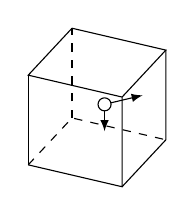
\begin{tikzpicture}
	\begin{axis}[axis lines = none, xlabel = x, ylabel=z, zlabel = y, xmax=2,ymax=2,zmax=2, xmin=-2, ymin=-2, zmin=-2, y post scale=-1, axis equal, ticks=none]
	\addplot3[draw=none] coordinates {(0,0,0)};
	\draw (axis cs:-1,1,-1)--(axis cs:1,1,-1)--(axis cs:1,1,1) -- (axis cs:-1,1,1)--(axis cs:-1,-1,1);
	\draw[dashed] (axis cs:-1,1,-1)--(axis cs:-1,-1,-1) -- (axis cs:1,-1,-1) ;
	\draw[dashed] (axis cs:-1,-1,-1)--(axis cs:-1,-1,1);
	\draw (axis cs:-1,1,-1)--(axis cs:-1,1,1);
	\draw (axis cs:-1,-1,1)--(axis cs:1,-1,1)--(axis cs:1,1,1);
	\draw (axis cs:1,1,-1)--(axis cs:1,-1,-1)--(axis cs:1,-1,1);
	\node[draw, circle, scale = .5] at (axis cs:.3,.3,.3) (N) {};
	\draw[-latex] (N) -- (.3,.3,-.3);
	\draw[-latex] (N) -- (.6,-.8,0);
	\end{axis}
	\end{tikzpicture}
\end{figure}
\begin{figure}[H]
	\begin{tikzpicture}
	\draw (-2,-2) -- (-2,2) -- (2,2) -- (2,-2) -- (-2,-2);
	\draw (0,0) circle (.25);
	\draw[thick] (-.1,-.25) -- (.1, -.25);
	\node[fill, circle, scale=.25, label = P] at (0,-.25) (P){};
	\draw[dashed] (P) -- (2*-.707, 2*-.707-.25) node[rotate={45}] {\varangle};
	\draw[dashed] (P) -- (2*.707, 2*-.707-.25) node {\textasteriskcentered};
	\draw[-latex] (P)--(0,-1-.25) node[label=n]{};
	\draw[-latex] (P) -- (.707,-.707-.25) node[label={r}] {};
	\draw[-latex] (P) -- (-.707,-.707-.25) node (r) {};
	
	\end{tikzpicture}	
\end{figure}
\begin{figure}[H]
	\begin{tikzpicture}[mark coordinate/.style={inner sep=0pt,outer sep=0pt,minimum size=3pt,
		fill=black,circle}]
	\def\R{2.5} % sphere radius
	\def\angEl{35} % elevation angle
	\def\angPhi{-90} % longitude of point P
	\def\step{20}
	\def\start{-20}
	%\LongitudePlane[pzplane]{\angEl}{\angPhi-20}
	%\path[pzplane] (10:\R) coordinate[mark coordinate] (B);
	%\LatitudePlane[oben]{\angEl}{10}
	%\LatitudePlane[unten]{\angEl}{-10}
	\filldraw[ball color=white] (0,0) circle (\R);
	\foreach \t in {-10,10} { \DrawLatitudeCircle[\R]{\t} }
	\foreach \i in {0,...,2}{ 
		\LongitudePlane[pzplane]{\angEl}{\angPhi+\start+\i*\step}
		\path[pzplane] (10:\R) coordinate[mark coordinate] (\i a);
		\path[pzplane] (-10:\R) coordinate[mark coordinate] (\i b);
	}
	\def\i{0}
	\draw (\i a)--(\i b);
	\foreach \d in {1,...,2} {
		\pgfmathtruncatemacro{\b}{\d - 1}
		\draw (\b b)--(\d a);
		\draw (\d a)--(\d b);
	}
	
%	\LongitudePlane[pzplane]{\angEl}{\angPhi}
%	\path[pzplane] (10:\R) coordinate[mark coordinate] (C);
%	\path[pzplane] (-10:\R) coordinate[mark coordinate] (D);
%	\LongitudePlane[pzplane]{\angEl}{\angPhi+20}
%	\path[pzplane] (10:\R) coordinate[mark coordinate] (E);
%	\path[pzplane] (-10:\R) coordinate[mark coordinate] (F);
%	\draw (A)--(B)--(C)--(D)--(E)--(F);
	
	\end{tikzpicture}
\end{figure}
%Kugle mit Dreiecken